\chapter{提案}
\par
本論文では,行動情報と発話情報の両方を活用する心的状態推定システムMultimodal Inference of Mind(MIoM)を提案する.MIoMは,人間の信念や行動,発話および人間が存在する環境の状態を基に心的状態を推定する.行動情報と発話情報の両方を心的状態の推定に活用することで,発話による行動の解釈の変化や行動による発話に解釈の変化を捉え,行動情報と発話情報の相互作用を考慮して心的状態を推定する.

\par
MIoMは,環境の状態や人間の心的状態を部分的に観測可能なマルコフ決定過程(POMDP)として表される.各時刻おける人間の信念や行動,発話および人間が存在する環境の状態をベイズの定理に適用し,人間が観測できていない環境領域についての信念と欲求を逐次的に推定する.


\section{関連研究との相違点}
\par
MIoMと関連研究との相違点は,行動情報と発話情報の両方を活用したマルチモーダルな心的状態推定を行う点である.MIoMは,行動情報と発話情報の両方を活用して心的状態を推定することで,発話による行動の解釈の変化や行動による発話の解釈の変化を捉え,行動情報と発話情報の相互作用を考慮した推定が可能となる.MIoMは,関連研究における問題点を解消するシステムとなっている.


\section{アルゴリズム}
\par
MIoMのシステム構成を図\ref{fig:sys_arc}に示す.

\begin{figure}[htbp]
  \begin{center}
    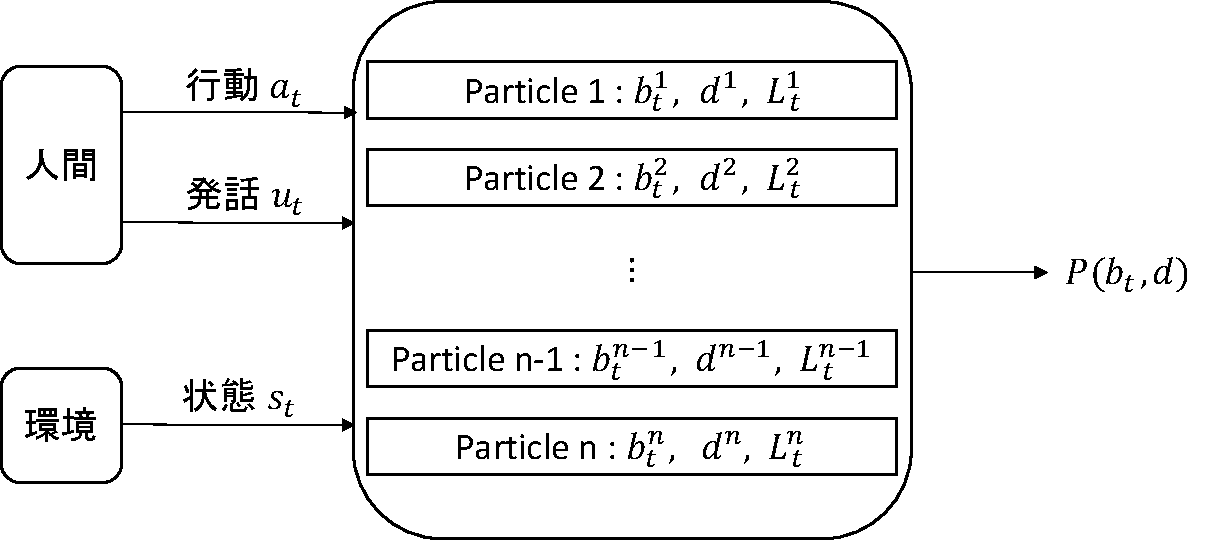
\includegraphics[scale=0.85]{./bt1.pdf}
    \caption{MIoMのシステム構成}
    \label{fig:sys_arc}
  \end{center}
\end{figure}
